\chapter{Sèries de Dirichlet}\label{capítol 1: sèries de Dirichlet}
Com hem vist abans, si volem estudiar el teorema dels primers en les progressions aritmètiques, necessitarem estudiar més a fons les sèries que va estudiar
Dirichlet.
\dfe{Sèrie de Dirichlet}{Una sèrie de Dirichlet és una sèrie de la forma
\[
\sum_{n\in\NN}\frac{f(n)}{n^s}
\]
On $f\colon\NN\rightarrow\CC$ és una funció aritmètica, i $s\in\CC$.
}
A partir d'ara, per simplificar la notació, sempre que tinguem $s\in\CC$, utilitzarem $\sigma$ per denotar la part real, i $t$ per denotar la part imaginària.\par

Ara farem un petit recopilatori de resultats de sèries:
\lema{Semiplà de convergència absoluta}{
\label{2.01_lema_semipla_de_convergencia_absoluta}Existeix un $\sigma_a\in\RR\cup\{\pm\infty\}$ tal que $\sum\frac{f(n)}{n^s}$ convergeix absolutament si 
$\Re(s)>\sigma_a$, i no ho fa si $\Re(s)<\sigma_a$. A aquest $\sigma_a$ se li dona el nom de ``$\sigma$ de convergència absoluta''.
}
\pf{
Si no hi ha cap $s$ tal que la sèrie convergeixi, aleshores $\sigma_a\coloneq+\infty$.\\
Si hi ha algun $s$ tal que $\sum\frac{f(n)}{n^s}$ convergeixi, considerem un $s'$ tal que $\sigma'>\sigma$. Aleshores volem veure que $\sum\frac{f(n)}{n^{s'}}$
convergeix:
\[
\left|\frac{f(n)}{n^{s'}}\right|=\frac{|f(n)|}{n^{\sigma'}}\leq\frac{|f(n)|}{n^{\sigma}}=\left|\frac{f(n)}{n^s}\right|
\]
I per tant, pel teorema de comparació, tenim que $\sum\frac{f(n)}{n^s}$ convergeix absolutament en un semiplà. Per tant, si considerem l'ínfim $\sigma$ que
funciona, tenim el que volíem demostrar.
}
Fins ara hem fet una mica la vista grossa pel que fa a la convergència d'un productori com el que va estudiar Euler. 
\dfe{Convergència de productoris}{
Sigui $\{z_n\}_n\subset\CC$ una successió de complexos, aleshores el productori $\prod z_n$ convergeix si i només si existeix el límit
$\lim_{n\rightarrow\infty}\prod_{i=1}^nz_n$, i aquest és no nul.
}
Donat que tenim un morfisme conegut que envia el producte a la suma, podem mirar com es tradueix el que acabem de definir al món de les sèries:
\lema{}{
Sigui $\{z_n\}_\NN\subset\CC$ on $\Re(z_n)>0$\footnote{Notem que el fet que el productori convergeixi implica que hi ha una quantitat finita lluny de 1, i per
tant, no és restrictiu suposar que tots són positius.}. Aleshores, $\prod z_n$ convergeix si i només si $\sum \log (z_n)$ convergeix.
}
\pf{
$\prod z_n$ convergeix $\iff$ $\log\left(\prod z_n\right)$ convergeix $\iff$ $\sum\log(z_n)$ convergeix; que és el que volíem veure.
}
Ara, amb aquest lema, passarem la noció de convergència absoluta de sumatoris a convergència absoluta de productoris:
\dfe{Convergència absoluta de productoris}{
Donada una seqüència $z_n$ amb $\Re(z_n)>0$, aleshores el productori $\prod z_r$ es diu que convergeix absolutament si $\sum \log(z_r)$ convergeix absolutament.
}
I és immediat veure que la convergència absoluta implica la convergència ordinària.\par

Ara donarem una altre lema que ens anirà ajudant al llarg del curs, ja que ens servirà per intercanviar productoris per sumatoris, que els tenim molt més 
controlats. I notem de fet, que la hipòtesis que $\Re(z_n)>-1$ no és gens restrictiva, ja que és una condició necessària per la convergència.
\lema{}{Si prenem $\{u_n\}_{\NN}\subset\CC$, amb $\Re(z_n)>-1$, aleshores:
\[
\sum_{n\geq 1}\log(1+u_n)\text{ convergeix absolutament}\iff\sum u_n\text{ convergeix absolutament}
\]
}
\claim{Si $|u|<\half$, aleshores $\half|u|\leq|\log(1+u)|
\leq\frac{3}{2}|u|$}
\pf{Notem que en aquest entorn, $\log(1+u)=u+\half u^2+\dots$. Primer demostrarem la primera desigualtat:
\begin{align*}
    \half|u|\leq& |\log(1+u)|=\left|u+\half u^2+\dots\right|\impliedby\\
    \half|u|\leq&|u|-\left|\half u^2+\frac{1}{3}u^3+\dots\right|\iff\\
    \half|u|\geq&\left|\half u^2+\frac{1}{3}u^3+\dots\right|\impliedby\\
    \half|u|\geq&\half|u|^2+\half|u|^3+\dots\impliedby\\
    \frac{|u|}{1-|u|}\leq&1\iff |u|\leq 1-|u|\iff|u|\leq \half
\end{align*}

Pel que fa a la segona desigualtat, notem que:
\begin{align*}
    \frac{3}{2}|u|\geq&|\log(1+u)|=\left|u+\half u^2 +\frac{1}{3}u^3+\dots\right|\impliedby\\
    \frac{3}{2}|u|\geq&|u|+\half|u|^2+\dots\impliedby\\
    \half|u|\geq&\half|u|^2+\half|u|^3+\dots\iff\\
    1\geq&\frac{|u|}{1-|u|}\iff\\
    1-|u|\geq&{|u|}\iff1\geq2|u|\iff\half\geq|u|
\end{align*}
Que és el que volíem veure.}

Per tant, per demostrar el lemma:
\pf{Notem que si $\sum_{n\geq 1}\log(1+u_n)$ convergeix absolutament, aleshores $u_n\rightarrow0$, per tant, només hi ha una quantitat petita amb valor absolut 
major que $\half$, per tant, pel criteri de comparació pel pas al límit tenim:
\[
\left|\log(1+u_n)\right|\geq\half\left|u_n\right|
\]
Per tant, la sèrie dels logaritmes convergeix absolutament, també ho fa la sèrie de les $u_n$. I per un argument idèntic, utilitzant l'altra desigualtat, 
obtenim l'altra implicació.
}
Ara que tenim una eina per transformar productoris a sumatoris, ens podem preguntar si hi ha alguna manera de transformar els sumatoris en productoris sobre els
primers (un producte d'Euler), que si més no, serà un dels objectes.
\Prop{Sèries de Dirichlet de funcions multiplicatives}{\label{2.02_proposició sèries de Dirichlet de funcions multiplicatives}Sigui $g\colon\NN\rightarrow\CC$ 
multiplicativa ($g(ab)=g(a)g(b)$ si $a$ i $b$ són coprimers). Suposem també que $\sum _\NN g(n)$ és absolutament convergent, aleshores:
\begin{enumerate}
    \ii $\prod_p 1+g(p)+g(p^2)+\dots$ és absolutament convergent, i $\prod_p 1+g(p)+g(p^2)+\dots=\sum_\NN g(n)$.\\
    \ii Si a més, $g$ és completament multiplicativa ($g(ab)=g(a)g(b)$ per tot $a$ i $b$), aleshores podem simplificar el productori, i tenim: 
    $\prod_p\frac{1}{1-g(p)}=\sum_\NN g(n)$
\end{enumerate}
}
\pf{Primer mirem que aquest productori convergeix a la sèrie.\\
Notem que per $N\in\ZZ_{\geq 2}$, definim $P(N)=\prod_{p\leq N}1+g(p)+g(p^2)+\dots=\sum_{n\in A(N)}g(n)$ on 
$A(N)\coloneq\{n\in\NN\text{ tal que tots els divisors primers }p\text{ de }n\text{ són }p\leq N\}$. Considerem
\[
\left|\sum_{\NN}g(n)-P(N)\right|=
\left|\sum_{\substack{n\in\NN\\n\text{ té algun }\\\text{divisor primer}\geq N}}g(n)\right|\leq
\left|\sum_{n\geq N}g(n)\right|\leq
\sum_{n\geq N}|g(n)|\xrightarrow{N\rightarrow\infty}0 
\]
On al final hem utilitzat que la sèrie $\sum_\NN g(n)$ convergeix.

Per parlar de convergència absoluta, utilitzarem finalment el lema d'abans, per tant, prenem $u_n=g(p)+g(p^2)+\dots$:
\[\sum_{p\leq N}\left|g(p)+g(p^2)+\dots\right|\leq\sum_{p\leq N}|g(p)|+|g(p^2)|+\dots\leq\sum_{n\geq 1}|g(n)|\]
Aquest últim pas és degut a que passem de sumar només sobre les potències dels primers a sobre tots els enters, però això sabem per hipòtesis que convergeix,
per tant, tot convergeix de manera absoluta.

Per veure la segona part de la proposició, només hem de veure que $g(p^k)=g(p)^k$, i per tant, tenim una sèrie geomètrica.

Una última observació abans de donar per demostrada la proposició, pel lema necessitem que $\Re(u_n)>-1$, però com que la sèrie dels $g(n)$ convergeix, tot se
n'ha d'anar a 0.
}
Ara utilitzarem aquesta proposició més general pel cas particular de les funcions de Dirichlet:
\coro{}{\label{2.03_corol·lari de sèries de Dirichlet multiplicatives a productes d'Euler}
Considerem $\sum_{n\geq1}\frac{f(n)}{n^s}$, amb $\sigma$ de convergència $\sigma_a$.\\
Si $f$ és multiplicativa, i $\sigma>\sigma_a$, tenim un producte d'Euler de la següent forma:
\[\sum_{n\geq 1}\frac{f(n)}{n^s}=\prod_{p}1+\frac{f(p)}{p^s}+\frac{f(p^2)}{p^{2s}}+\dots\]
I si a més, $f$ és completament multiplicativa, aleshores podem simplificar les coses encara més:
\[
\sum_{n\geq 1}\frac{f(n)}{n^s}=\prod_p\frac{1}{1-\frac{f(n)}{n^s}}
\]
}

\pf{
Si $f$ és multiplicativa (o completament multiplicativa), aleshores podem aplicar la proposició \ref{2.02_proposició sèries de Dirichlet de funcions multiplicatives}, i ens dona el que volem.
}
\exemple{
Per $\zeta(s)=\sum_{n\geq1}\frac{1}{n^{s}}$ té com a $\sigma_a=1$, i per tant, per tot $s$ amb part real major que 1, podem expressar $\zeta(s)=\prod_p(1-p^{-s})\inv$.
}

Ara donarem un mètode per calcular sumatoris:
\teorema{Criteri de sumació d'Abel}{\label{2.04_teorema_sumació_Abel}Sigui $a\colon\NN\rightarrow\CC$, considerem $A(t)\coloneq\sum_{n\leq t}a(n)$ les sumes parcials de $a$; i una funció $g:\RR_{\geq0}\rightarrow\CC$ amb derivada contínua en un interval $[x,y]\neq\varnothing$\footnote{Per alguna raó, al professor li ha agradat considerar l'interval $[y,x]$, però em nego a fer servir aquesta notació.}. Aleshores 
\[
\sum_{x<n\leq y}a(n)g(n)=A(y)g(y)-A(x)g(x)-\int_x^yA(t)g'(t)\dd t
\]
}
\pf{
\[
\sum_{x<n\leq y}a(n)g(n)=\sum_{n=\lfloor x\rfloor+1}^{\lfloor y\rfloor}(A(n)-(A(n-1)))g(n)=\sum_{n=\lfloor x\rfloor+1}^{\lfloor y\rfloor}A(n)g(n)-\sum_{n=\lfloor x\rfloor}^{\lfloor y\rfloor-1}A(n)g(n+1)=
\]
I ara si ho tornem a agrupar tot:
\[
=A(\lfloor y\rfloor)g(\lfloor y\rfloor)-A(\lfloor x\rfloor)g(\lfloor x\rfloor+1)+\sum_{n=\lfloor x\rfloor+1}^{\lfloor y\rfloor-1}A(n)(g(n)-g(n+1))
\]
I si ara substituïm $g(n)-g(n+1)=-\int_{n}^{n+1}g'(t)\dd t$:
\[
=A(\lfloor y\rfloor)g(\lfloor y\rfloor)-A(\lfloor x\rfloor)g(\lfloor x\rfloor+1)-\sum_{n=\lfloor x\rfloor+1}^{\lfloor y\rfloor-1}A(n)\int_{n}^{n+1}g'(t)\dd t
\]
I com que en cada interval $A(n)$ és constant, podem entrar-ho dins de la integral:
\[
=A(\lfloor y\rfloor)g(\lfloor y\rfloor)-A(\lfloor x\rfloor)g(\lfloor x\rfloor+1)-\sum_{n=\lfloor x\rfloor+1}^{\lfloor y\rfloor-1}\int_{n}^{n+1}A(t)g'(t)\dd t
\]
I això ho podem posar tot en un sol tros:
\[
=A(\lfloor y\rfloor)g(\lfloor y\rfloor)-A(\lfloor x\rfloor)g(\lfloor x\rfloor+1)-\int_{\lfloor x\rfloor+1}^{\lfloor y\rfloor}A(t)g'(t)\dd t
\]
Per simplificar aquest desastre, notem que $A$ és constant en $[x,\lfloor x\rfloor+1]$ i en $[\lfloor y \rfloor+1,y]$, per tant
\[
=A(\lfloor y\rfloor)g(\lfloor y\rfloor)-A(\lfloor x\rfloor)g(\lfloor x\rfloor+1)-\int_{x}^{y}A(t)g'(t)\dd t+\int^{\lfloor x\rfloor+1}_x A(t)g'(t)\dd t+\int_{\lfloor y \rfloor}^y A(t)g'(t)\dd t
\]
\[
=A(\lfloor y\rfloor)g(\lfloor y\rfloor)-A(\lfloor x\rfloor)g(\lfloor x\rfloor+1)-\int_{x}^{y}A(t)g'(t)\dd t+A(\lfloor x\rfloor )\int^{\lfloor x\rfloor+1}_xg'(t)\dd t+A(\lfloor y \rfloor)\int_{\lfloor y \rfloor}^yg'(t)\dd t
\]
I ara aquestes integrals sí que les sabem fer:
\[
=A(\lfloor y\rfloor)g(\lfloor y\rfloor)-A(\lfloor x\rfloor)g(\lfloor x\rfloor+1)+A(\lfloor x\rfloor )(g(\lfloor x\rfloor+1)-g(x))+A(\lfloor y \rfloor)(g(y)-g(\lfloor y\rfloor))-\int_{x}^{y}A(t)g'(t)\dd t
\]
I ara movem una mica els dits (recordem que $A(x)=A(\lfloor x\rfloor)$, i que $A(y)=A(\lfloor y\rfloor)$), i diem avada kedabra i tot el que no volem mor:
\[=A(y)g(y)-A(x)g(x)-\int_x^y A(t)g'(t)\dd t\]
Que és el que volíem veure.
}
Una mica d'intuïció darrere d'aquest teorema, és que quan tens una sèrie que té moltes cancel·lacions, i que per tant, les $A(n)$ no creix massa; aleshores multiplicar per una funció $g$ no canvia tant això com poder seria d'esperar, ja que tot es pot posar en termes de les $A$.

\lema{Fita tècnica}{\label{2.05_lema_fita_de_sèries_de_Dirichlet} Suposem que $\sum_{n\geq 1} \frac{f(n)}{n^{s_0}}$ té sumes parcials fitades en $s_0\in\CC$, és a dir: existeix una fita $M\in\RR_{\geq 0}$ tal que $\left|\sum_{n\leq x}\frac{f(n)}{n^s_0}\right|\leq M$ per $x\geq 1$, aleshores per $s\in\CC$ tal que $\sigma>\sigma_0$ tenim:
\[
\left|\sum_{a< n\leq b}\frac{f(n)}{n^s}\right|\le2Ma^{\sigma_0-\sigma}\left(1+\frac{|s-s_0|}{\sigma-\sigma_0}\right)
\]
}
\pf{
Per aplicar el teorema de sumació d'Abel hem d'agafar la $a$ i la $g$, i donat que tenim controlades les sumes parcials de $\frac{f(n)}{n^s}$ és raonable prendre-la com a $a(n)=\frac{f(n)}{n^S}$, i deixar que $g(t)=t^{s_{0}-s}$. I això ens deixa:
\begin{align*}    
\left|\sum_{a<n\leq b}\frac{f(n)}{n^{s_0}}\right|=\left|A(b)g(b)-A(a)g(a)-\int_a^bA(t)g'(t)\dd t\right|\leq\\
\leq |A(b)||g(b)|+|A(a)||g(a)|+\int_a^b M \left|\left(t^{s_0-s-1}\right)(s_0-s)\right| \dd t\leq\\
\leq Mb^{s_0-s}+Ma^{s_0-s}+M|s_0-s|\int_{a}^b\left|t^{s_0-s-1}\right|\dd t
\end{align*}
Ara hi ha 2 observacions que podem fer per tenir una fita més polida. La primera és que per hipòtesis $\sigma>\sigma_0$ i per tant, $|\sigma_0-\sigma|=\sigma-\sigma_0$ i com que $b>a$, tenim que $b^{s_0-s}<a^{s_0-s}$. I una altra observació que es pot fer és que $\left|t^{s_0-s-1}\right|=t^{\sigma_0-\sigma-1}$. Introduint tots aquests canvis a l'expressió ens queda:
\[
2Ma^{s_0-s}+M|s-s_0|\left(\frac{a^{\sigma_0-\sigma}-b^{\sigma_0-\sigma}}{\sigma-\sigma_0}\right)\leq2Ma^{\sigma_0-\sigma}+M|s-s_0|\frac{2a^{\sigma_0-\sigma}}{\sigma-\sigma_0}=2Ma^{\sigma_0-\sigma}\left(1+\frac{|s-s_0|}{\sigma-\sigma_0}\right)
\]
}
Fins ara ens hem interessat sobre tot per la convergència absoluta (per exemple amb el lema \ref{2.01_lema_semipla_de_convergencia_absoluta}). Ara veurem la relació que hi ha entre això i la convergència normal i corrent:
\lema{Semiplà de convergència}{
\label{2.06_lema_semipla de convergencia} Donada una sèrie de Dirichlet $\sum_{n\geq1}\frac{f(n)}{n^s}$, aleshores aquesta convergeix si i només si $\sigma>\sigma_c$ per alguna $\sigma_c\in\RR\cup\{\pm\infty\}$. De la mateixa manera que abans, aquesta $\sigma_c$ rep un nom: es diu $\sigma$ de convergència.
}
\pf{
La demostració és molt similar a la del lema \ref{2.01_lema_semipla_de_convergencia_absoluta}. Si no hi ha cap tal $s_0$ convergent, aleshores $\sigma_c\coloneq+\infty$. Sinó, sigui $s_0$ un complex que faci convergir la sèrie. Considerem ara un $s$ tal que $\s>\s_0$. Anomenem $M$ una fita de les sumes parcials de $\sum \frac{f(n)}{n^s}$. Aleshores:
\[
\left|\sum_{a<n\leq b}\frac{f(n)}{n^s}\right|\leq2Ma^{\sigma_0-\sigma}\left(1+\frac{|s-s_0|}{\s-\s_0}\right)\leq Ka^{\s_0-\s}\xrightarrow{a\rightarrow\infty}0
\]
Que és el que volíem veure.
}
I ara poder ve la pregunta natural de quina diferència hi ha entre $\s_a$ i $\s_c$. Podria ser que un fos finit i l'altre no? Podria ser que fossin sempre el mateix (com és el cas amb la convergència d'una sèrie de potències en els complexos)? Doncs resulta que de fet, els dos valors sempre estan molt a prop:
\Prop{Distància entre $\sigma_c$ i $\sigma_a$}{\label{2.07_proposició}
Suposem que tenim una sèrie de Dirichlet $\sum_{n\geq 1}\frac{f(n)}{n^s}$ amb $\s_c$ finit, aleshores la $0\leq\s_a- \s_c\leq1$.
}
\pf{
Suposem que $\sum_{n\geq 1}\frac{f(n)}{n^s}$ és convergent per un $s_0$. Volem veure que és convergent absolutament per $s_1$ si $\s_1>\s_0+1$. Però que $s_0$ sigui convergent ens diu que existeix una fita $A\in\RR_{\geq0}$ tal que $\left|\frac{f(n)}{n^s}\right|\leq A$ $\forall n \geq 1$. Aleshores:
\[
\left|\frac{f(n)}{n^{s_1}}\right|=\left|\frac{f(n)}{n^{s_0}}\right|\left|n^{s_0-s_1}\right|\leq An^{s_0-s_1}
\]
Per tant, com que $s_1-s_0>1$, tenim que $\sum_{n\geq 1}n^{s_0-s_1}$ convergeix. I per tant pel criteri de comparació, tenim que la sèrie convergeix per $s_1$. Que és el que volíem veure.
}
Ara volem veure que tota sèrie de Dirichlet és una funció analítica (de fet meromòrfica). I per això veurem el següent teorema, que ens ajudarà a controlar les sèries de Dirichlet. 
\teorema{Límit d'una successió de funcions holomorfes és holomorfa.}{\label{2.08_teorema}Sigui $\mcal U\in\CC$ un obert i sigui $\{f_n\}_n$ una successió de funcions holomorfes $f_n\colon\mcal U\rightarrow \CC$, que convergeixen sobre tot compacte $K$ de $\mcal U$ cap a una funció $f$. Aleshores:
\begin{enumerate}
    \ii $f$ és holomorfa.\\
    \ii $\{f_n'\}_n$ convergeix uniformement sobre tots els compactes cap a $f'$.
\end{enumerate}}
\pf{
Sigui $D$ un disc contingut en $\mcal U$. Sigui $z_0\in D^\mathrm{o}$.\\

Com que $f_n$ és holomorfa, pel teorema de Cauchy:
\[
f_n(z_0)=\frac{1}{2\pi i}\int_{\partial D}\frac{f_n(z)}{z-z_0}\dd z
\]
I per tant, aplicant el límit tenim
\[
f(z_0)=\lim_{n\rightarrow\infty}f_n(z_0)=\lim_{n\rightarrow\infty}\frac{1}{2\pi i}\int_{\partial D}\frac{f_n(z)}{z-z_0}\dd z
\]
Però com que $f_n$ convergeix uniformement, podem entrar el límit dins de la integral:
\[
f(z_0)=\frac{1}{2\pi i}\int_{\partial D}\lim_{n\rightarrow\infty}\frac{f_n(z)}{z-z_0}\dd z=\frac{1}{2\pi i}\int_{\partial D}\frac{f(z)}{z-z_0}\dd z
\]
Però ara pel teorema de Morera (que bàsicament diu el revers del teorema de Cauchy) ens diu que $f$ és holomorfa.\\

Per veure la segona part del teorema, utilitzarem un argument idèntic però amb:
\[
f_(z_0)^{(j)}=\frac{j!}{2\pi i}\int_{\partial D}\frac{f(z)}{(z-z_0)^{j+1}}\dd z
\]
}
I ara com que totes les sumes parcials són funcions analítiques, seria molt bonic que ara aquestes funcions convergissin de manera uniforme sobre tots els compactes: així podríem aplicar aquest teorema i veuríem que les sèries de Dirichlet són analítiques. Que és justament el que farem:
\Prop{Les sèries de Dirichlet convergeixen de manera uniforme sobre tot compacte}{\label{2.09_proposició}
Una sèrie de Dirichlet $\sum_{n\geq 1}\frac{f(n)}{n^s}$ convergeix uniformement sobre tot compacte a l'interior del semiplà de convergència.
}
\pf{
Tot compacte de $\CC$ està contingut en un rectangle (com que està acotat podem posar-lo dins d'una bola, i aquesta pot anar a dins d'un rectangle). Per tant, si veiem que l'enunciat és cert sobre rectangles, ja estarem.

Considerem un rectangle $R=[\alpha,\beta]\times[\gamma,\delta]$ amb $\alpha>\s_c$. Sigui ara $s\in R$ i considerem $s_0=\s_0\in\RR$ tal que $\s_c<\s_0<\alpha\leq\s=\Re(s)$. Definim $M$ com una fita de les sumes parcials de $|\sum_{n\leq x}\frac{f(n)}{n^{s_0}}|$. Volem fitar $|\sum_{a<n\leq b}\frac{f(n)}{n^s}|$ per una cosa que no depengui de $s$. Aplicant el \ref{2.05_lema_fita_de_sèries_de_Dirichlet}:
\[
\left|\sum_{a<n\leq b}\frac{f(n)}{n^s}\right|\leq 2 M a^{\sigma_0-\sigma}\left(1+\frac{|s-s_0|}{\sigma-\sigma_0}\right)
\]
Però notem que $\s-\s_0$ i $|s-s_0|$ estan fitats dins del rectangle, siguin $A$ i $B$ les seves fites. Aleshores podem introduir-ho a la nostra fita, i deixar-ho independent de $s$:
\[
\left|\sum_{a<n\leq b}\frac{f(n)}{n^s}\right|\leq 2 M a^{B}\left(1+\frac{A}{B}\right)
\]
Si anomenem $C=2M(1+\frac{A}{B})$, i observem que $B<0$, aleshores;
\[
\left|\sum_{a<n\leq b}\frac{f(n)}{n^s}\right|\leq Ca^B\xrightarrow{a\rightarrow\infty}0
\]
Que és el que volíem veure.
}
I ara demostrarem el que volíem: que tota sèrie de Dirichlet és una funció holomorfa en tot un semiplà.
\coro{Les sèries de Dirichlet són funcions holomorfes}{\label{2.10_corol·lari}Considerem la sèrie de Dirichlet $F(s)=\sum_{n\geq1}\frac{f(n)}{n^s}$, aleshores $F$ és una funció holomorfa per tot $\sigma>\sigma_c$.\\
I a més, $F'(s)=-\sum_{n\geq1}\frac{f(n)\log(n)}{n^s}$ per $\s >\s_c$.}
\pf{
Considerem $F_N(s)=\sum_{n=1}^N\frac{f(n)}{n^S}$, aleshores per la proposició \ref{2.09_proposició}, $F_N\rightrightarrows F$ sobre tot compacte $K$ del semiplà de convergència. A més, com que $F_N$ són sumes finites de funcions holomorfes, són funcions holomorfes. Per tant pel teorema \ref{2.08_teorema} $F$ és una funció holomorfa, i té per derivada $F'(s)=-\sum_{n\geq1}\frac{f(n)\log(n)}{n^s}$. Que és el que volíem veure.
}
Ara acabem de veure que, igual que les sèries de potències, les sèries de Dirichlet són funcions holomorfes; i ara veurem una altra semblança:
\Prop{Teorema d'unicitat}{\label{2.11_proposició}
Siguin $F(s)=\sum_{n\geq1}\frac{f(n)}{n^s}$ i $G(s)=\sum_{n\geq1}\frac{g(n)}{n^s}$ sèries de Dirichlet. Sigui $\s_0=\max\{\s_a^F,\s_a^G\}$ i suposem que existeix una successió $(s_k)_{k\geq1}$ al semiplà $\s>\s_0$ tals que $F(s_k)=G(s_k)$ i $\lim_{k\rightarrow\infty}\s=\infty$, llavors:
\[f(n)=g(n)\quad \forall n\in\NN\]
}
\pf{
Notem que en tenim prou amb veure que $H(s)\coloneq\sum_{n\geq1}\frac{h(n)}{n^s}$ amb $H(s_k)=0$, aleshores això implica que $h(n)=0$ per tot $n$.(aquí la idea és considerar $H=F-G$).\\
Per tant, suposem que hi ha algun $N\geq1$ tal que $h(N)\neq0$, i sense pèrdua de generalitat podem assumir que tal $N$ és mínim. Aleshores:
\[
H(s)=\frac{h(N)}{N^s}+\sum_{n\geq N+1}\frac{h(n)}{n^s}
\]
I movent una mica les coses:
\[
h(N)=\left(H(s)-\sum_{n\geq N+1}\frac{h(n)}{n^s}\right)N^s
\]
I si avaluem en $s_k$:
\[
h(N)=\left(\cancelto{0}{H(s_k)}-\sum_{n\geq N+1}\frac{h(n)}{n^s}\right)N^s=-N^s\sum_{n\geq N+1}\frac{h(n)}{n^s}
\]
Notem que com que $\lim_{k}\s\rightarrow\infty$, aleshores $\min_k \s_k$ està ben definit i és estrictament més gran que $\s_0$ i per tant prenem $c\in(\s_0,\min_k\s_k)$.\\
Ara, el nostre objectiu és veure que $h(N)=0$, i per veure-ho fitarem superiorment aquest terme:
\[
|h(N)|\leq N^{\s_k}\sum_{k\geq N+1}\frac{|h(n)|}{n^{\s_k}}=N^{\s_k}\sum_{k\geq N+1}\frac{|h(n)|}{n^cn^{s_k-c}}\leq\frac{N^{\s_k}}{(N+1)^{\s_k}}\frac{1}{(N+1)^{-c}}\sum_{n\geq N+1}\frac{|h(n)|}{n^c}
\]
Notem que $\frac{1}{(N+1)^{-c}}\sum_{n\geq N+1}\frac{|h(n)|}{n^c}$ convergeix independentment de $k$, per tant, podem substituir-ho per $C$:
\[
|h(N)|\leq \left(\frac{N}{N+1}\right)^{s_k}C\xrightarrow{k\rightarrow\infty}0
\]
Per tant, pel lema del sandvitx tenim que $h(N)=0$, però això contradiu les hipòtesis que teníem.
}

I d'aquí en podem treure un corol·lari immediat:
\coro{}{
\label{2.12_coro semipla sense zeros}Sigui $F(s)=\sum_{n\geq1}\frac{f(n)}{n^s}$ i suposem que existeix algun $s_0$ amb $\sigma_0>\sigma_a$ tal que $F(s_0)\neq0$, aleshores el conjunt de zeros és finit, i per tant, hi ha algun semiplà en que la funció no s'anul·la.}
\pf{
Notem que si hi haguessin infinits $s_k$ tals que $F(s_k)=0$, aleshores pel teorema d'unicitat: $f(n)=0$, però això contradiu el fet que $F(s_0)=0$.
}
I continuant amb la motivació d'abans: les semblances entre les sèries de potències i les de Dirichlet són encara més estretes del que semblen. Per exemple, de la mateixa manera en que el radi de convergència d'una sèrie de potències és la distància a la singularitat més propera, també hi ha una cosa similar amb sèries de Dirichlet amb coeficients positius:
\teorema{Landau}{\label{2.13_teorema_landau}Sigui $F(s)=\sum_{n\geq1}\frac{f(n)}{n^S}$ una sèrie de Dirichlet que convergeix per $\sigma>c\in\RR$. Si a més, tenim:
\begin{enumerate}
    \ii Que $f(n)\in\RR_{\geq0}$ per tota $n\geq n_0$,\\
    \ii i suposem que $F(s)$ estén a una funció holomorfa en un disc al voltant de $c$.
\end{enumerate}
Aleshores, $F(s)$ convergeix per $\s>c-\varepsilon$ per alguna $\varepsilon>0$.

}
I abans d'anar a la demostració del teorema, considerem què passa si $F$ estén de manera meromorfa (però no holomorfa) en $s_0$:
\coro{Extensions meromorfes}{\label{2.14_corol·lari}
Suposem que $F(s)=\sum_{n\geq1}\frac{f(n)}{n^s}$, i suposem que $f(n)\in\RR_{\geq0}$ per tot $n>n_0$, i $f$ admet continuació meromorfa en un disc al voltant de $s=\sigma_c$, aleshores $F(s)$ té un pol en $s=\s_c$.
}
\pf{
Per demostrar aquest corol·lari notem que si $F$ estén en un disc a una funció meromorfa però $\sigma_c$ no és un pol, aleshores podem reduir la mida del disc fins a que no li quedin pols i pel teorema \ref{2.13_teorema_landau} tenim que estén una mica cap a l'esquerra, i per tant la sèrie convergeix en algun $\sigma<\sigma_c$ però això és una contradicció. Per tant tenim que $F$ ha de tenir un pol en $\sigma_c$.
}
I ara, entenent la motivació, del teorema:\\
\begin{wrapfigure}{r}{0.3\textwidth}
\begin{center}
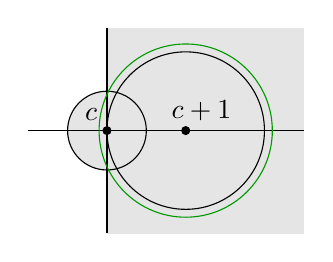
\begin{tikzpicture}
    \filldraw[color=black!10!white] (0,-1.3)--(0,1.3)--(2.5,1.3)--(2.5,-1.3)--(0,-1.3);
    \filldraw[color=black!10!white] (0,0) circle (0.5);
    \draw (-1,0)--(2.5,0);
    \draw (0,-1.3)--(0,1.3);
    \draw (0,0) circle (0.5);
    \filldraw (0,0) circle (0.05);
    \draw (-0.2,0.2) node {$c$};
    \draw (1,0) circle (1);
    \draw (1.2,0.25) node {$c+1$};
    \filldraw (1,0) circle (0.05);
    \draw[color=black!40!green] (1,0) circle (1.1);
\end{tikzpicture}
\caption{\label{fig:thm13}La zona pintada de gris és la zona en que $F$ és holomorfa.}
\end{center}

\end{wrapfigure}
\pf{
    

Notem que si considerem $F$ com una sèrie de potències al voltant de $c+1$, és fàcil veure que tenim $R>1$ (si mirem a la figura \ref{fig:thm13}, el que diem és que al cercle verd centrat a $c+1$, la funció és holomorfa).
\[
F(s)=\sum_{k\geq0}\frac{F^{(k)}(c+1)}{k!}(s-(c+1))^k
\]
I pel corol·lari 10, tenim que
\[
F^{(k)}(c+1)=(-1)^k\sum_{n\geq1}\frac{f(n)(\log(n))^k}{n^{c+1}}
\]
I substituint això a l'equació de dalt:
\[
F(s)=\sum_{k\geq0}\sum_{n\geq1}\frac{f(n)(\log n)^k(c+1-s)^k}{k!n^{c+1}}
\]
Com que ho tenim per $R>1$ sabem que $F$ ha de convergir per $s=c-\varepsilon$ per algun $\varepsilon>0$:
\begin{align*}
    F(c-\varepsilon)&=\sum_{k\geq0}\sum_{n\geq1}\frac{f(n)(\log n)^k(1+\varepsilon)^k}{k!n^{c+1}}
\end{align*}
Notem que com que $f(n)\geq0$, ens diu que convergència $\implies$ convergència absoluta $\implies$ podem reordenar:
\begin{align*}
    F(c-\varepsilon)&=\sum_{k\geq0}\sum_{n\geq1}\frac{f(n)(\log n)^k(1+\varepsilon)^k}{k!n^{c+1}}=\\
    &=\sum_{n\geq1}\sum_{k\geq0}\frac{f(n)(\log n)^k(1+\varepsilon)^k}{k!n^{c+1}}=\\
    &=\sum_{n\geq1}\frac{f(n)}{n^{c+1}}\sum_{k\geq0}\frac{(\log n)^k(1+\varepsilon)^k}{k!}=\\
    &=\sum_{n\geq1}\frac{f(n)}{n^{c+1}}e^{\log(n)(1+\eps)}=\\
    &=\sum_{n\geq1}\frac{f(n)}{n^{c+1}}n^{1+\eps}=\\
    &=\sum_{n\geq1}\frac{f(n)}{n^{\eps-c}}
\end{align*}
Per tant, com que $F(c-\eps)$ convergeix com a sèrie de potències, també ho fa com a sèrie de Dirichlet, i per tant, $\s_c<c$, que és el que volíem veure.
}
Es podria dir que hi ha una sèrie de Dirichlet d'especial importància: la funció $\zeta(s)$ de Riemann, degut al seu problema del mil·lenni que té associat: trobar els zeros a la franja $0<\sigma<1$. Però tal com l'hem definit, aquesta pregunta no té sentit, així que ara veurem com la podem estendre:
\teorema{Riemann}{\label{2.15_teorema_extensió_de_riemann}La funció $\zeta(s)=\sum_{n\geq1}\frac{1}{n^s}$ estén a una funció meromorfa a $\s>0$ com
\[
\zeta(s)\coloneq\frac{1}{s-1}+\phi(s)\quad \text{on }\phi(s)\text{ és una funció holomorfa per }\s>0. 
\]}
\pf{
Per $\s>1$ tenim, gràcies al corol·lari \ref{2.03_corol·lari de sèries de Dirichlet multiplicatives a productes d'Euler} $\zeta(s)$ es pot expressar:
\[
\zeta(s)=\sum_{n\ge1}\frac{1}{n^s}=\sum_{n\geq1}n\left(\frac{1}{n^s}-\frac{1}{(n+1)^s}\right)=\sum_{n\geq1}n\int_{n}^{n+1}sx^{-s-1}\dd x=s\int_1^{\infty}\lfloor x\rfloor x^{-s-1}\dd x
\]
I ara podem separar la integral en 2 trossos, utilitzant que $\lfloor x \rfloor=x-\{x\}$ on $\{x\}$ és la part fraccionària de $x$.
\[
s\int_1^\infty xx^{-1-s}\dd x=s\int_1^\infty x^{-s}\dd x=\left.-s\frac{x^{-s+1}}{s-1}\right|_1^\infty=\frac{s}{s-1}=1-\frac{1}{s-1}
\]
Per tant, el que queda és:
\[
\phi(s)\coloneq1-s\int_1^\infty \{x\}x^{-s-1}\dd x
\]
I hem de veure que $\phi$ és holomorfa. Per fer-ho utilitzarem la següent claim:
\claim{
Veure que la integral $1-s\int_1^\infty \{x\}x^{-s-1}\dd x$ convergeix uniformement pels $\sigma\geq\delta>0$ és suficient per veure que convergeix a una funció holomorfa.
}
\pf{Per veure això, notem que la successió de funcions $I_n(s)=1-s\int_1^N \{x\}x^{-s-1}\dd x$ són holomorfes, ja que es poden expressar com a un sumatori $\sum_{n\geq1}\int_n^{n+1}(x-n)x^{-s-1}\dd x$, i totes aquestes són funcions holomorfes: per tant, si hi ha convergència uniforme sobre qualsevol compacte, el límit és una funció holomorfa: però si ho fa en un semiplà obert, ho farà sobre qualsevol compacte d'aquest.}
I ara tornem a la demostració. Primer fitarem aquesta integral de tal manera que no depengui de $\s$, i que només ho faci de $\delta$: Fixem un $\varepsilon>0$, aleshores, prenem $r(\eps)=\frac{1}{\left(\delta\varepsilon\right)^{\frac{1}{\delta}}}$ tal que $\forall r>r(\eps)$ la integral 
\[
\left|\int_r^\infty\frac{\{x\}}{x^{1+s}}\dd x\right|<\eps\qquad \text{per tot }\s\geq\delta.
\]
Però notem que:
\[
\left|\int_r^\infty\frac{\{x\}}{x^{1+s}}\dd x\right|\leq\int_r^\infty\frac{|\{x\}|}{\left|x^{1+s}\right|}\dd x<\int_r^\infty\frac{1}{x^{1+s}}\dd x=\left.\frac{x^{-\s}}{-\s}\right|_{r}^{\infty}=\frac{1}{\s r^{\s}}\leq\frac{1}{\delta r^\delta}=r(\eps)
\]
Per tant, per tot $\eps$ hi ha un $r(\eps)$ que no depèn de $s$ tal que la cua de la integral és petita: que és el que volíem veure.
}
I a partir del que acabem de veure, sabem que $\zeta$ té un pol en $s=1$ de residu 1, per tant:
\coro{}{\label{2.16_coro comportament de zeta en s=1}La funció $\zeta$ té un pol de residu 1; i per tant:
\[
\lim_{s\rightarrow1^+}\frac{\log(\zeta(s))}{\log(\frac{1}{1-s})}=1
\]
On $s\in\RR_{\geq1}$
}
\pf{
La part que el residu és 1, és immediat veient que $\zeta(s)=\frac{1}{s-1}+\phi(s)$. Pel que fa a que $\lim_{s\rightarrow1^+}\frac{\log(\zeta(s))}{\log(\frac{1}{1-s})}=1$, només hem de veure que $\zeta(s)\sim \frac{1}{s-1}$ a $s=1$; per tant, $\log(\zeta(s))\sim\log(\frac{1}{z-1})$, que és el que volíem veure.
}
I un altre corol·lari que ve mitjanament inspirat del teorema \ref{2.15_teorema_extensió_de_riemann}:
\coro{}{\label{2.17_coro sèries de potències de p}
La sèrie
\[\lim_{\substack{s\rightarrow1\\s\in\RR_{\geq1}}}\frac{\sum_{p}\frac{1}{p^s}}{\log(\frac{1}{s-1})}=1\]
És a dir: $\sum_p\frac{1}{p^s}\sim-\log(s-1)$ amb $s$ a prop de $1$.\\
I a més:
\[
\sum_p\sum_{k\ge2}\frac{1}{p^{ks}}<1\qquad \text{per tot }s\in\RR_{\geq1}
\]
}
\pf{
Recordem que $\zeta(s)=\prod_p(1-p^{-s})\inv$ per $\s>1$; per tant, per $s\in\RR_{\geq1}$ tenim que
\[
\log(\zeta(s))=-\sum_p\log\left(1-\frac{1}{p^s}\right)=\sum_p\left(\sum_{k\geq0}\frac{1}{kp^{ks}}\right)
\]
Aquest últim pas és l'expansió de Taylor del logaritme al voltant de $s=1$.
\[
\sum_p\left(\sum_{k\geq0}\frac{1}{kp^{ks}}\right)=\sum_p\left(\sum_{k\geq2}\frac{1}{kp^{ks}}\right)+\sum_p\frac{1}{p^s}
\]
Notem que en $s=1$ aquesta suma no convergeix. Per tant, si veiem la segona part del corol·lari, això implicarà la primera. Per tant, ara procedirem a demostrar la segona part:
\begin{align*}
    \sum_p\sum_{k\geq2}\frac{1}{kp^{ks}}&\leq\sum_p\sum_{k\geq2}\frac{1}{p^{ks}}=\sum_{p}\frac{1}{p^{2s}}\sum_{k\geq0}\frac{1}{p^{ks}}=\sum_p\frac{p^{-2s}}{1-\frac{1}{p^s}}=\\
    &=\sum_p\frac{1}{p^s}\frac{1}{p^{s}-1}\leq\sum_p\frac{1}{p(p-1)}<\sum_{n\geq1}\frac{1}{n(n-1)}=\\
    &=\sum_{n\geq1}\frac{1}{n-1}-\frac{1}{n}=1
\end{align*}
Que és el que volíem veure.
}